\chapter{Chapter 1: Let's Start with the
Bootloader}\label{ch-bootloader}

\section{Introduction}\label{introduction}

The first piece to start with when writing an operating system's kernel
is the \emph{boot loader} which is the code that is responsible for
loading the main kernel from the disk to the main memory so the kernel
can be executed. Before getting started in the details of the boot
loader and all other parts of the kernel, we need to learn a little bit
about the tools (e.g.~compilers and programming languages) that we will
use in our journey of creating a kernel. In this chapter, we start with
an overview on the tools and their basics and then we start in writing a
boot loader.

\section{x86 Assembly Language
Overview}\label{x86-assembly-language-overview}

To build a boot loader, we need to use assembly language, also, there
are some parts of an operating system kernel that cannot be written in a
high-level language and assembly language should be used instead as you
will see later in this book, therefore, a basic knowledge of the target
architecture assembly is required, in our case, the target architecture
of our kernel is x86.

The program that takes a source code which is written in assembly
language and transforms this code to the machine language is known as
\emph{assembler} \footnote{While the program that transforms the source
  code which is written in high-level language such as C to machine code
  is known as \emph{compiler}.}. There are many assemblers available for
x86 but the one that we are going to use is Netwide Assembler (NASM).
However, the concepts of x86 assembly are the same, they are tight to
the architecture itself, also the instructions are the same, so if you
grasp the basics it will be easy to use any other assembler \footnote{Another
  popular open-source assembler is GNU Assembler (GAS). One of main
  differences between NASM and GAS that the first uses Intel's syntax
  while the second uses AT\&T syntax.} even if it uses other syntax than
NASM. Don't forget that the assembler is just a tool that helps us to
generate an executable x86 machine code out of an assembly code, so, any
suitable assembler that we use to reach our goal will be enough.

In this section I don't aim to examine the details of x86 or NASM, you
can consider this section as a quick start on both x86 and NASM, the
basics will be presented to make you familiar with x86 assembly
language, more advanced concepts will be presented later when we need
them. If you are interested in x86 assembly for its own sake, there are
multiple online resources and books that explain it in details.

\subsection{Registers}\label{registers}

In any processor architecture, and x86 is not an exception, a register
is a small memory inside the processor's chip. Like any other type of
memories (e.g.~RAM), we can store data inside a register and we can read
data from it, the registers are too small and too fast. The processor
architecture provides us with multiple registers. In x86 there are two
types of registers: general purpose registers and special purpose
registers. In general purpose registers we can store any kind of data we
want, while the special purpose registers are provided by the
architecture for some specific purposes, we will encounter the second
type later in our journey of creating 539kernel.

x86 provides us with eight general purpose registers and to use them in
order to read from or write to them we refer to them by their names in
assembly code. The names of these registers are: \lstinline!EAX!,
\lstinline!EBX!, \lstinline!ECX!, \lstinline!EDX!, \lstinline!ESI!,
\lstinline!EDI!, \lstinline!EBP!, and \lstinline!ESP!. While the
registers \lstinline!ESI!, \lstinline!EDI!, \lstinline!EBP! and
\lstinline!ESP! are considered as general purpose registers in x86
architecture \footnote{According to Intel's manual.}, we will see later
that they store some important data in some cases and it's better to use
them carefully if we are forced to.

The size of each one of x86's general purpose registers is
\lstinline!32! bits (\lstinline!4! bytes) and due to that, they are
available only on x86 processors that supports \lstinline!32-bit!
architecture \footnote{Also they are available on \textbf{64-bit} x86
  CPUs such as Core i7 for instance.} such as Pentium 4 for instance.
These \lstinline!32-bit! registers are not available on x86 processors
that support only \lstinline!16-bit! architecture or lower, so, for
example, you can't use the register \lstinline!EAX! in Intel 8086
because it is a \lstinline!16-bit! x86 processor and not
\lstinline!32-bit!.

In old days, when \lstinline!16-bit! x86 processors were dominant,
assembly programmers used the registers \lstinline!AX!, \lstinline!BX!,
\lstinline!CX! and \lstinline!DX! and each one of them is of size
\lstinline!16! bits (\lstinline!2! bytes), but when \lstinline!32-bit!
x86 processors came, these registers have been extended to have the size
\lstinline!32-bit! and their names were changed to \lstinline!EAX!,
\lstinline!EBX!, \lstinline!ECX! and \lstinline!EDX!. The first letter
\lstinline!E! of the new names means \emph{extended}. However, the old
names are still usable in \lstinline!32-bit! x86 processors and they are
used to access and manipulate the first \lstinline!16! bits of the
corresponding register, for instance, to access the first \lstinline!16!
bits of the register \lstinline!EAX!, the name \lstinline!AX! can be
used. Furthermore, the first \lstinline!16! bits of these registers can
be divided into two parts and each one of them is of size \lstinline!8!
bits (\lstinline!1! bytes) and has its own name that can be referred to
in the assembly code. The first \lstinline!8! bits of the register are
called the \emph{low} bits, while the second \lstinline!8! bits are
called the \emph{high} bits.

Let's take one of these register as an example:\lstinline!AX! register
is a \lstinline!16-bit! register which is a part of the bigger
\lstinline!32-bit! \lstinline!EAX! register in \lstinline!32-bit!
architecture. \lstinline!AX! \footnote{Or in other words for
  \lstinline!32-bit! architecture: The first \lstinline!16! bits of
  \lstinline!EAX!.} is divided into two more parts, \lstinline!AL! for
the \textbf{l}ow \lstinline!8! bits as the second letter of the name
indicates and \lstinline!AH! for the \textbf{h}igh \lstinline!8! bits as
the second letter of the name indicates. The same division holds true
for the registers \lstinline!BX!, \lstinline!CX! and \lstinline!DX!,
figure \ref{fig:26012022_0} illustrates that division.

\begin{figure}
\centering
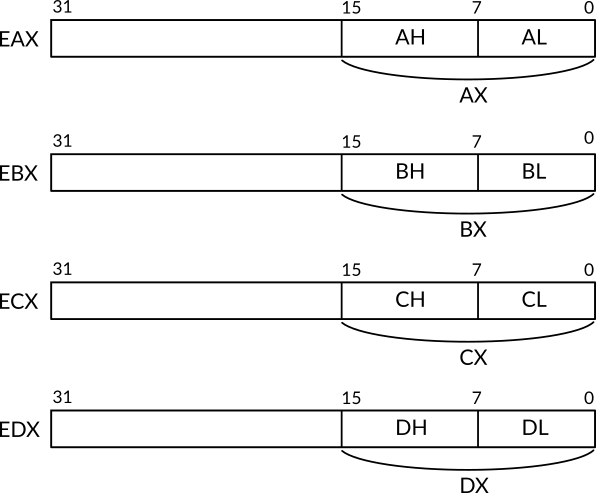
\includegraphics[width=0.50000\textwidth]{Figures/bootloader-ch/Fig26012022_0.png}
\caption{How the Registers \lstinline!EAX!, \lstinline!EBX!,
\lstinline!ECX! and \lstinline!EDX! are Divided in
x86}\label{fig:26012022_0}
\end{figure}

\subsection{Instruction Set}\label{instruction-set}

The processor's architecture provides the programmer with a bunch of
\emph{instructions} that can be used in assembly code. Processor's
instructions resemble functions \footnote{Or a procedure for people who
  work with Algol-like programming languages.} in a high-level languages
which are provided by the libraries, in our case, we can consider the
processor as the ultimate library for the assembly code. As with
functions in high-level programming languages, each instruction has a
name and performs a specific job, also, it can take parameters which are
called \emph{operands}. Depending on the instruction itself, the
operands can be a static value (e.g.~a number), a register name that the
instruction is going to fetch the stored value of it to be used or even
a memory location.

The assembly language is really simple. An assembly code is simply a
sequence of instructions which will be executed sequentially. The
following is an example of assembly code, don't worry about its
functionality right now, you will understand what it does eventually.

\begin{lstlisting}
mov ah, 0Eh
mov al, 's' 
int 10h
\end{lstlisting}

As you can see, each line starts with an instruction which is provided
to us by x86 architecture, in the first two lines we use an instruction
named \lstinline!mov! and as you can see, this instruction receives two
operands which are separated by a comma. In the current usage of this
instruction we can see that the first operand is a register name while
the second operand is a static value. The third line uses another
instruction named \lstinline!int! which receives one operand. When this
code is running, it will be executed by the processor sequentially,
starting from the first line until it finishes in the last line.

If you are interested on the available instructions on x86, there is a
four-volumes manual named ``Intel® 64 and IA-32 architectures software
developer's manual'' provided by Intel that explains each instruction in
details \footnote{\url{https://software.intel.com/en-us/articles/intel-sdm}}.

\subsubsection{\texorpdfstring{Assigning Values with
\texttt{mov}}{Assigning Values with mov}}\label{assigning-values-with-mov}

You can imagine a register as a variable in high-level languages. We can
assign values to a variable, we can change its old value and we can copy
its value to another variable. In assembly language, these operations
can be performed by the instruction \lstinline!mov! which takes the
value of the second operand and stores it in the first operand. You have
seen in the previous examples the following two lines that use
\lstinline!mov! instruction.

\begin{lstlisting}
mov ah, 0Eh
mov al, 's' 
\end{lstlisting}

Now you can tell that the first line copies the value \lstinline!0Eh! to
the register \lstinline!ah!, and the second line copies the character
\lstinline!s! to the register \lstinline!al!. The single quotation is
used in NASM to represent strings or characters and that's why we have
used it in the second line, based on that, you may noticed that the
value \lstinline!0Eh! is not surrounded by a single quotation though it
contains characters, in fact, this value isn't a string, it is a number
that is represented by hexadecimal numbering system and due to that the
character \lstinline!h! was put in the end of that value, that is,
putting \lstinline!h! in the end of \lstinline!0E! tells NASM that this
value is a hexadecimal number, the equivalent number of \lstinline!0E!
in the decimal numbering system, which we humans are using, is
\lstinline!14!, that is \lstinline!0E! and \lstinline!14! are the
exactly the same, but they are represented in two different numbering
system\footnote{Numbering systems will be discussed in more details
  later.}.

\subsection{NASM}\label{nasm}

Netwide Assembler (NASM) is an open-source assembler for x86
architecture which uses Intel's syntax of assembly language, the other
well-known syntax for assembly language is AT\&T syntax and, of course,
there are some differences between the two, the first syntax is used in
the official manuals of Intel. NASM can be used through command line to
assemble \footnote{The process of transforming an assembly source code
  to machine code is known as \emph{assembling}.} x86 assembly code and
generate the corresponding machine code. The basic usage of NASM command
is the following.

\begin{lstlisting}
nasm -f <format> <filename> [-o <output>]
\end{lstlisting}

The argument \lstinline!format! decides the binary format of the
generated machine code, the binary format will be discussed in more
details in a moment. The second argument is the \lstinline!filename! of
the assembly file that we would like to assemble, and the last option
and argument are optional, we use them if we want to specify a specific
name for the generated binary file, the default name will be same as the
filename with a different extension.

\subsubsection{Binary Format}\label{binary-format}

A \emph{binary format} is basically a specification which gives a
blueprint of how a binary file is organized, in other words, it
describes how a binary file is structured, in general there are multiple
parts in a binary file and a binary format can be used format them, the
machine code is one part of a binary file parts. Note that each
executable file uses some binary format to organize its content and to
make a specific operating system understands its content. There is no
difference between the programming languages in the matter of the binary
format \footnote{Of course the programming language should be a
  \emph{compiled} programming language such as C and Rust and not an
  \emph{interpreted} such as Python or a one that uses a virtual machine
  such as Java.} that will be used in the last output of the compiling
process, for example in Linux, if we create a software either by C, Rust
or assembly, the last executable result will be a binary file that is
formatted by using a binary format known as \emph{Executable and
Linkable Format} (ELF) which is the default in Linux. There are many
other binary formats, Mach-O is one example which is used by Mach-based
\footnote{Mach is an operating system's kernel which is well-known for
  using \emph{microkernel} design. It has been started as a research
  effort in Carnegie Mellon University in 1985. Current Apple's
  operating systems macOS and iOS are both based on an older operating
  system known as NeXTSTEP which used Mach as its kernel,}, another
example is Portable Executable (PE) which is used by Microsoft Windows.

Each operating system knows its own binary format well, and knows how a
binary file that uses this format is structured, and how to seek the
binary file to find the machine code that should be loaded into memory
and executed by the processor. For example, when you run an ELF
executable file in GNU/Linux system, the Linux kernel knows it is an ELF
executable file and assumes that it is organized in a specific way, by
using the specification of ELF, Linux kernel will be able to locate the
machine code of the software inside the ELF file and load it into memory
to be ready for execution.

In any binary format, one major part of the binary file that uses this
format is the machine code that has been produced by compiling or
assembling some source code, the machine code is specific to a processor
architecture, for example, the machine code that has been generated for
x64 \footnote{The x86 architecture that supports 64-bit.} cannot run on
x86. Because of that the binary files are distributed according to the
processor architecture which can run on, for example, GNU/Linux users
see the names of software packages in the following format
\lstinline!nasm_2.14-1_i386.deb!, the part \lstinline!i386! tells the
users that the binary machine code of this package is generated for
\lstinline!i386! architecture, which is another name for x86 by the way,
that means this package cannot be used in a machine that uses ARM
processor such as Raspberry Pi for example.

Due to that, to distribute a binary file of the same software for
multiple processor's architectures, a separate binary file should be
generated for each architecture, to solve this problem, a binary format
named \lstinline!FatELF! was presented. In this binary format, the
software machine code of multiple processor architectures are gathered
in one binary file and the suitable machine code will be loaded and run
based on the type of the system's processor. Naturally, the size of the
files that use such format will be bigger than the files that uses a
binary format that is oriented for one processor architecture. Due to
the bigger size, this type of binary formats is known as \emph{fat
binary}.

Getting back to the \lstinline!format! argument of NASM, if our goal of
using assembly language is to produce an executable file for Linux for
example, we will use \lstinline!elf! as a value for \lstinline!format!
argument. But we are working with low-level kernel development, so our
binary files should be flat and the value of \lstinline!format! should
be \lstinline!bin! to generate a \emph{flat binary} file which doesn't
use any specification, instead, in flat binary files, the output is
stored as is with no additional information or organization, only the
output machine language of our code. Using flat binary for bootloader
does make sense and that's because the code which is going to load
\footnote{Which is BIOS as we will see later.} our binary file doesn't
understand any binary format to interpret it and fetch the machine code
out of it, instead, the content of the binary file will be loaded to the
memory as is.

\section{GNU Make}\label{gnu-make}

GNU Make is a build automation tool. Well, don't let this fancy term
make you panic! the concept behind it is too simple. When we create a
kernel of an operating system \footnote{Or any software with any other
  compiled programming languages.} we are going to write some assembly
code and C code and both of them need to be assembled and compiled (for
the C code) to generate the machine code as binary files out of them.
With each time a modification is made in the source code, you need to
recompile (or reassemble) the code over and over again through writing
the same commands in the terminal in order to generate the last binary
output of your code. Beside the compiling and recompiling steps, an
important step needs to take place in order to generate the last output,
this operation is known as \emph{linking}, usually a programming project
contains multiple source files that call each other, compiling each one
of these files is going to generate a separate \emph{object file}
\footnote{An object file is a machine code of a source file and it is
  generated by the compiler. The object file is not an executable file
  and in our case at least it is used to be linked with other object
  files to generate the final executable file.} for each one, in linking
process these different object files are linked with each other to
generate one binary file out of these multiple object files, this last
binary file represents the program that we are writing.

These operations which are needed to generate the last binary file out
of the source code is known as \emph{building process}, which, as
mentioned earlier, involves executing multiple commands such as
compiling, assembling and linking. The building process a tedious job
and error-prone and to save our time (and ourselves from boredom of
course) we don't want to write all these commands over and over again in
order to generate the last output, we need an alternative and here where
GNU Make \footnote{And any other building automation tool.} comes to the
rescue, it \emph{automates} the \emph{building} process by gathering all
required commands in a text file known as \lstinline!Makefile! and once
the user runs this file through the command \lstinline!make!, GNU Make
is going to run these commands sequentially, furthermore, it checks
whether a code file is modified since the last building process or not,
if the case is that the file is not modified then it will not be
compiled again and the generated object file from the last building
process is used instead, which of course minimize the needed time to
finish the building process.

\subsection{Makefile}\label{makefile}

A \lstinline!makefile! is a text file that tells GNU Make what are the
needed steps to complete the building process of a specific source code.
There is a specific syntax that we should obey when writing
\lstinline!makefile!. A number of \emph{rules} may be defined, we can
say that a \lstinline!makefile! has a list of rules that define how to
create the executable file. Each rule has the following format:

\begin{lstlisting}[language=make]
target: prerequisites
    recipe
\end{lstlisting}

When we run the command \lstinline!make! without specifying a defined
target name as an argument, GNU Make is going to start with the first
rule in the \lstinline!makefile! only if the first rule's target name
doesn't start with dot, otherwise, the next rule will be considered. The
name of a target can be a general name or filename. Assume that we
defined a rule with the target name \lstinline!foo! and it's not the
first rule in \lstinline!makefile!, we can tell GNU Make to execute this
rule by running the command \lstinline!make foo!. One of well-known
convention when writing a \lstinline!makefile! is to define a rule with
target name \lstinline!clean! that deletes all object files and binaries
that have been created in the last building process. We will see after a
short time the case where the name of a target is a filename instead of
general name.

The \lstinline!prerequisites! part of a rule is what we can call the
list of dependencies, those dependencies can be either filenames (the C
files of the source code for instance) or other rules in the same
\lstinline!makefile!. For GNU Make, to run the a specific rule
successfully, the dependencies of this rule should be fulfilled, if
there is another rule in the dependencies, it should be executed
successfully first, if there is a filename in the dependencies list and
there is no rule that has the same filename as a target name, then this
file will be checked and used in the recipe of the rule.

Each line in the \lstinline!recipe! part should start with a tab and it
contains the commands that is going to run when the rule is being
executed. These commands are normal Linux commands, so in this part of a
rule we are going to write the compiling commands to compile the C
source files, assembling commands for the assembly source files and
linking command that links the generated object files. Any arbitrary
command can be used in the recipe as we will see later when we create
the \lstinline!makefile! of 539kernel. Consider the following C source
files, the first one is \lstinline!file1.c!, the second one is
\lstinline!file2.h! and the third one is \lstinline!file2.c!.

\begin{lstlisting}[language=C]
#include "file2.h"
int main()
{
    func();
}
\end{lstlisting}

\begin{lstlisting}[language=C]
void func();
\end{lstlisting}

\begin{lstlisting}[language=C]
#include <stdio.h>
void func()
{
    printf( "Hello World!" );
}
\end{lstlisting}

By using these three files, let's take an example of a
\lstinline!makefile! with filenames that have no rules with same
target's name.

\begin{lstlisting}[language=make]
build: file1.c file2.c
    gcc -o ex_file file1.c file2.c
\end{lstlisting}

The target name of this rule is \lstinline!build!, and since it is the
first and only rule in the \lstinline!makefile! which its name doesn't
start with a dot, then it will be executed directly once the command
\lstinline!make! is issued, another way to execute this rule is by
mentioning its name explicitly as an argument to \lstinline!make!
command as the following: \lstinline!make build!.

The rule \lstinline!build! depends on two C files, \lstinline!file1.c!
and \lstinline!file2.c!, they should be available on the same directory.
The the recipe uses GNU GCC to compile and link these two files and
generate an executable file named \lstinline!ex_file!. The following is
an example of a \lstinline!makefile! that has multiple rules.

\begin{lstlisting}[language=make]
build: file2.o file1.o
    gcc -o ex_file file1.o file2.o
file1.o: file1.c
    gcc -c file1.c
file2.o: file2.c file2.h
    gcc -c file2.c file2.h
\end{lstlisting}

In this example, the first rule \lstinline!build! depends on two object
files \lstinline!file1.o! and \lstinline!file2.o!. Before running the
building process for the first time, these two files will not be
available in the source code directory \footnote{Since they are a result
  of one step of the building process which is the compiling step that
  has not been performed yet.}, therefore, we have defined a rule for
each one of them. The rule \lstinline!file1.o! is going to generate the
object file \lstinline!file1.o! and it depends on \lstinline!file1.c!,
the object file will be simple generated by compiling
\lstinline!file1.c!. The same happens with \lstinline!file2.o! but this
rule depends on two files instead of only one.

GNU Make also supports variables which can simply be defined as the
following: \lstinline!foo = bar! and they can be used in the rules as
the following: \lstinline!$(foo)!. Let's now redefine the second
\lstinline!makefile! by using the variables.

\begin{lstlisting}[language=make]
c_compiler = gcc
buid_dependencies = file1.o file2.o
file1_dependencies = file1.c
file2_dependencies = file2.c file2.h
bin_filename = ex_file
build: $(buid_dependencies)
    $(c_compiler) -o $(bin_filename) $(buid_dependencies)
file1.o: $(file1_dependencies)
    gcc -c $(file1_dependencies)
file2.o: $(file2_dependencies)
    gcc -c $(file2_dependencies)
\end{lstlisting}

\section{The Emulators}\label{the-emulators}

While developing an operating system kernel, for sure, you will need to
run that kernel to test your code frequently. That's of course can be
done by writing the image of the kernel on a bootable device and reboot
you machine over and over again in order to run your kernel. Obviously,
this way isn't practical and needs a lot of chore work. Moreover, when a
bug shows up, it will be really hard to debug your code by using this
way. An alternative better way is to use an emulator to run your kernel
every time you need to test it.

An emulator is a software that acts like a full computer and by using it
you can run any code that require to run on a bare metal hardware. Also,
by using an emulator, everything will be virtual, for example, you can
create a virtual hard disk (that is, not real) that can be used by your
kernel, this virtual hard disk will be a normal file in you host system,
so, if anything goes wrong in your code you will not lose your data in
your main system. Furthermore, an emulator can provide you with a
debugger which will make your life a lot easier when you need to debug
your code.

There are two options for the emulator, QEMU \footnote{\url{https://www.qemu.org/}}
and Bochs \footnote{\url{https://bochs.sourceforge.io/}}. Both of them
are open source and both of them provides us with a way to run a
debugger. Personally, I liked Bochs' debugger better since it provides
an easy GUI that saves a lot of time. QEMU on the other hand, gives that
user the ability to use GNU Debugger through command line. Running a
kernel image is simple in QEMU, the following command performs that.

\begin{lstlisting}
qemu-system-x86_64 kernel.img
\end{lstlisting}

Where \lstinline!kernel.img! is the binary file of the kernel and the
bootloader. You will see later in 539kernel's \lstinline!Makefile! that
the option \lstinline!-s! is used with QEMU, it can be safely removed
but it is used to make GNU debugger able to connect to QEMU in order to
start a debugging session. Of course you can find a lot more about QEMU
in its official documentation \footnote{\url{https://www.qemu.org/docs/master/}}.

To run your kernel by using Bochs, you need to create a configuration
text file named \lstinline!bochsrc!. Each time you run Bochs it will use
this configuration file which tells Bochs the specifications of the
virtual machine that will be created, these specifications are something
about the virtual processors, their number, their available feature, the
number of available virtual disks, their options, the path of their
files and so on. Also, whether the debugger of Bochs and its GUI is
enabled or not are decided through this configuration file. This
configuration can be easily created or edited by using a command line
interface through running the command \lstinline!bochs! with no
arguments. After creating the file you can use the option
\lstinline!-f bochsrc! where \lstinline!bochsrc! is the filename of the
configuration file to run your kernel directly with no question from
Bochs about what to do.

\section{Writing the Boot Loader}\label{writing-the-boot-loader}

When a computer powers on, a piece of code named bootloader is loaded
and takes the control of the computer. Usually, the goal of the
bootloader is loading the kernel of an operating system from the disk to
the main memory and gives the kernel the control over the computer. The
firmware of a computer is the program which loads the bootloader, in
IBM-compatible computers the name of this firmware is BIOS (Basic
Input/Output System) \footnote{Before the advent of UEFI.}.

There is a place in the hard disk called \emph{boot sector}, it is the
first sector of a hard disk \footnote{As we will see later, a magnetic
  hard disk has multiple stacked \emph{platters}, each platter is
  divided into multiple \emph{tracks} and inside each track there are
  multiple \emph{sectors}.}, BIOS loads the content of the boot sector
as a first step of running the operating system. Loading the boot
sector's content means that BIOS reads the content from hard disk and
loads it into the main memory (RAM). This loaded content from the boot
sector should be the bootloader, and once its loaded into the main
memory, the processor will be able to execute it as any other code that
we use in our computers. So, the last step performed by BIOS in booting
process is giving the control to the bootloader to do whatever it wants.

Before getting started in writing 539kernel, we need to write the
bootloader that is going to load 539kernel from the disk. In
IBM-compatible PCs that uses BIOS to perform the booting process, the
size of the bootloader is limited to \lstinline!512! bytes and due to
this limited size and the need of using low-level services, the
bootloader is usually written in assembly language, also, because of
this limited size, we cannot depend on BIOS to load 539kernel instead of
the bootloader and that's because a kernel is usually bigger than
\lstinline!512! bytes, therefore, a small bootloader is loaded by BIOS
in order to load the bigger piece of code which is the kernel. The
reason of this limited size of the bootloader is because of the size of
a sector in the hard disk itself. Each sector in the hard disk has the
size of \lstinline!512! bytes and as we have mentioned, BIOS is going to
load the content of the first sector of hard disk, the boot sector,
which, of course, as any other sector its size is \lstinline!512! bytes.

Beside the bootloader's limited size, it is going to run on an \emph{x86
operating mode} known as \emph{real mode} \footnote{The concept of x86
  operating modes and the real mode will be discussed in more details
  later.}, what we need to know about that for now is that real mode is
a \lstinline!16-bit! environment, so, even if the working processor is a
\lstinline!64-bit! processor, we can only use \lstinline!16-bit!
features of the processor, such as the registers of size \lstinline!16!
bits.

The booting process is too specific to the computer architecture as we
have seen and it may differs between one architecture and another. Some
readers, especially computer science students may notice that the
academic textbooks of operating systems don't mention the bootloader or
discuss it.

\subsection{Hard Disk Structure}\label{hard-disk-structure}

A hard disk consists of multiple \emph{platters} which are stacked
together one above the other, have you ever seen a CD or a DVD? A
platter has exactly the same shape, refer to Figure \ref{fig:a-platter}.
The both surfaces (top and down) of a platter are covered by a magnetic
layer which stores the data. For each surface of a platter there is a
read/write head on it, and as you guessed, the role of this head is to
read from a surface or write to it, a head is attached to an arm. Those
arms move horizontally, back and forth, and because the other end of all
of those arms are attached to the same physical part, they will be moved
back and forth together to the same location at the same time. Figure
\ref{fig:platters-arms-heads} shows how the platters, arms and
read/write heads are assembled together.

\begin{figure}
\centering
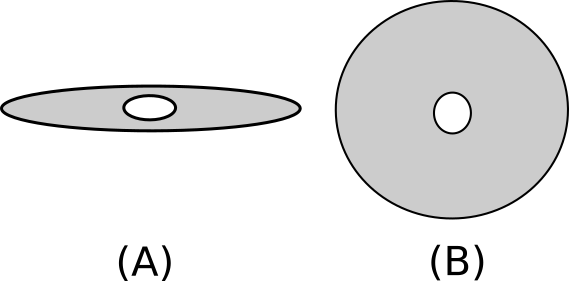
\includegraphics[width=0.50000\textwidth]{Figures/bootloader-ch/a-platter.png}
\caption{(A) Shows a platter when we see it from the side. (B) Shows a
platter when we see it from top/down.}\label{fig:a-platter}
\end{figure}

A surface of a platter is divided into a number of tracks and each track
is divided into a number of sectors. In Figure \ref{fig:tracks-sectors}
you can see how tracks and sectors are organized on a surface, the gray
circles that have the same center (cocenteric) are the tracks, a track
consists of a smaller parts which called sectors. A sector is the
smallest unit that holds data in hard disks and as you know from our
previous discussion, the first sector in a hard disk is known as boot
sector.

\begin{figure}
\centering
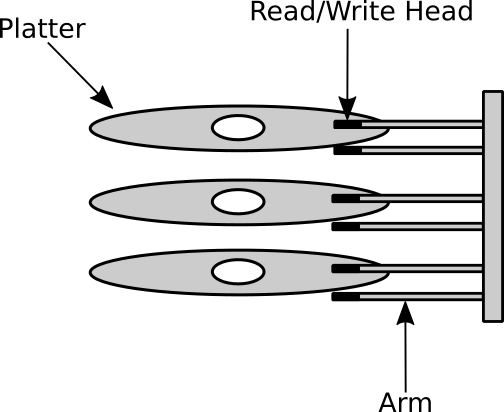
\includegraphics[width=0.50000\textwidth]{Figures/bootloader-ch/platters-arms-heads.png}
\caption{Shows how the parts of a hard disk are assembled
together.}\label{fig:platters-arms-heads}
\end{figure}

When a command is sent to the hard disk to write some data on it or read
from it, at least two mechanical moves \footnote{This fancy term
  \emph{mechanical moves} means that some physical parts of hard disk
  moves physically.} are performed. The first move is taken by the arms,
they move back or forth in order to be upon the track that contains the
data we would like to read, this operation is known as \emph{seek}
operation. So, \emph{seek time} is the time needed to put a specific
track under a read/write head. After finishing the seek operation, the
read/write head will be on the right track but, also, it will be on a
random sector \footnote{Not exactly random, can you tell why?}, to reach
the sector that we would like to read from (or write to) the platter
rotates until the read/write head becomes upon the required sector. The
speed of rotation is measured by a unit known as \emph{revolutions per
minute} (RPM) and the needed time to reach the required sector is known
as \emph{rotational latency}. Finally, the data will be
\emph{transferred} from the hard disk to the main memory, the time
needed to transfer a number of bits known as \emph{transfer time}.

Let's assume as an example a hard disk that has \lstinline!3! platters,
which means it has \lstinline!6! surfaces, arms and read/write head.
When the operating system request from the hard disk to seek a specific
track, for instance track \lstinline!3!, all \lstinline!6! heads will
seek the track \lstinline!3! and when the seek operation ends, the
\lstinline!6! heads will point to the same physical position on all
\lstinline!6! surfaces, that is, the top head of the first platter and
the bottom head of it will point to that same place, but the first one
on the top while the second is on the bottom, and so on for the other
\lstinline!4! remaining heads, the collection of all these tracks that
the heads point to at some point of time is called a \emph{cylinder}.

\begin{figure}
\centering
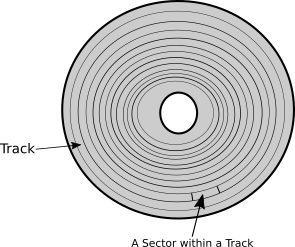
\includegraphics[width=0.50000\textwidth]{Figures/bootloader-ch/tracks-sectors.png}
\caption{Shows Tracks and Sectors on a platter's
surface.}\label{fig:tracks-sectors}
\end{figure}

Now, based on what we know about how a hard disk works, can we imagine
what happens inside the hard disk when BIOS loads a bootloader? First,
the arms will seek the track number \lstinline!0! \footnote{I didn't
  mention that previously, but yes, the bootloader resides in track
  \lstinline!0!.}, that is, the arms move back or forth until they reach
the track \lstinline!0!, then the platter rotates until the read/write
head become upon the sector \lstinline!0!, finally, the content of
sector \lstinline!0! is transferred to the main memory.

\subsection{BIOS Services}\label{bios-services}

We are in a journey of writing an operating system kernel, which means
that we are dealing with a little bit harsh environment! Do you remember
all libraries that we are lucky to have when developing normal software
(user-space software), well, none of them are available right now! And
they will not be available until we decide to make them so and work hard
to do that. Even the simple function \lstinline!printf! of C is not
available.

But that's fine, for our luck, in this environment, where there is too
little available for us to write our code, BIOS provides us with a bunch
of useful services that we can use in real mode, so, we can use these
services in our bootloader to get things done.

BIOS services are like a group of functions in high-level languages that
is provided by some library, each function does something useful and we
deal with those functions as black boxes, we don't know what's inside
these functions but we know what they do and how to use them. So,
basically, BIOS provides us a library of functions and we are going to
use some of these functions in our bootloader.

BIOS services are divided into categories, there are video services
category, disk services category, keyboard services category and so on.
Each category is identified by a unique number called \emph{interrupt
number}. In high-level world, we witnessed the same concept but with
different mechanism, for example, C standard library provides us with
many services (functions) such as input/output functions, string
manipulation functions, mathematical functions and so on, these
functions are categorized and each category is label by the
\emph{library name}, for example, all input/output functions can be
found in \lstinline!stdio.h! and so on. In BIOS, for example, the
category of video services has the interrupt number \lstinline!10h!. As
mentioned earlier, the letter\lstinline!h! after a number means that
this number represented in hexadecimal numbering system, or for short, a
hexadecimal number. Here, \lstinline!10h! doesn't equal the decimal
number \lstinline!10!. We already said that when a hexadecimal number is
mentioned we use \lstinline!h! as a postfix, also, \lstinline!0x!
\footnote{C programming language, for instance, uses this way for
  hexadecimal numbers.} can be used as a prefix instead of
\lstinline!h!, so \lstinline!10h! and \lstinline!0x10! are equivalents.

Inside each services category, there is a bunch of services, each one
can do a specific thing and they are identified by a number. Continuing
with C analogy, a service is a function labeled by a name (e.g.
\lstinline!printf!) and this function reside in a library (e.g.
\lstinline!stdio.h!) which is same as a category of services in BIOS. As
we said, the interrupt number \lstinline!10h! represents the category of
video services, and the service of printing a character on a screen
(function) is represented by the number \lstinline!0Eh!.

Interrupts is a fundamental concept in x86 architecture. What we need to
know about them right now is that they are a way to call a specific code
which is assigned to the interrupt number and calling an interrupt in
assembly is really simple, the instruction \lstinline!int! is used as
the following: \lstinline!int 10h!. That's it! We use the instruction
\lstinline!int! and gives it the interrupt number that represent the
code that we would like to call as an operand. In this example, we are
calling the code of interrupt \lstinline!10h! which is, as we mentioned
multiple time, the category of BIOS video services. When the CPU
executes this instruction, BIOS will be called and based on the
interrupt number it will know that we want to use one of available video
services, but which one exactly!

In the previous example, we actually didn't tell BIOS which video
service we would like to use and to do that we need to specify service
number in \lstinline!ah! register before calling the interrupt.

\begin{lstlisting}
mov ah, 0Eh
int 10h
\end{lstlisting}

That's it, all the BIOS services can be used in this exact way. First we
need to know what is the interrupt number that the service belongs to,
then, we need to know the number of the service itself, we put the
service number in the register \lstinline!ah! then we call the interrupt
by its number by using \lstinline!int! instruction.

The previous code calls the service of printing a character on a screen,
but is it complete yet? Actually no, we didn't specify what is the
character that we would like to print. We need something like parameters
in high-level languages to pass additional information for BIOS to be
able to do its job. Well, lucky us! the registers are here to the
rescue.

When a BIOS service needs additional information, that is, parameters.
It expects to find these information in a specific register. For
example, the service \lstinline!0Eh! in interrupt \lstinline!10h!
expects to find the character that the user wants to print in the
register \lstinline!al!, so, the register \lstinline!al! is one of
service \lstinline!0Eh! parameters. The following code requests from
BIOS to print the character \lstinline!S! on the screen:

\begin{lstlisting}
mov ah, 0Eh
mov al, 'S'
int 10h
\end{lstlisting}

\subsection{A Little Bit More of x86 Assembly and
NASM}\label{a-little-bit-more-of-x86-assembly-and-nasm}

We need to learn a couple more things about x86 assembly to be able to
start. In NASM, each line in the source code has the following format.

\begin{lstlisting}
label: instruction operands
\end{lstlisting}

The label is optional, the operands depend on x86 instruction in use, if
it doesn't get any operand then we don't need to write them. To write
comments on NASM we begin with semi-colon and write whatever we like
after it as a comment and the rest of the source line will be considered
as a part of the comment.

A label is a way to give an instruction or a group of instructions a
meaningful name, then we can use this name in other places in the source
code to refer to this instruction/group of instructions, we can use
labels for example to call this group of instructions or to get the
starting memory address of these instructions. Sometimes, we may use
labels to make the code more readable.

We can say that a label is something like the name of a function or
variable in C, as we know a variable name in C is a meaningful name that
represents the memory address of a location in the main memory that
contains the value of a variable, the same holds true for a function
name. Labels in NASM works in the same way, under the hood it represents
a memory address. The colon in label is also optional.

\begin{lstlisting}
print_character_S_with_BIOS:
    mov ah, 0Eh
    mov al, 'S'
    int 10h
\end{lstlisting}

You can see in the code above, we gave a meaningful name for the bunch
of instructions that prints the character \lstinline!S! on the screen.
After defining this label in our source code, we can use it anywhere in
the same source code to refer to this bunch of instructions.

\begin{lstlisting}
call_video_service int 10h
\end{lstlisting}

This is another example of labels. This time we eliminated the optional
colon in label's name and the label here points to only one instruction.
Please note that extra whitespaces and new lines doesn't matter in NASM,
so, the following is equivalent to the one above.

\begin{lstlisting}
call_video_service
    int 10h
\end{lstlisting}

Consider the following code, what do you think it does?

\begin{lstlisting}
print_character_S_with_BIOS:
    mov ah, 0Eh
    mov al, 'S'

call_video_service:
    int 10h
\end{lstlisting}

Still it prints \lstinline!S! on the screen. Introducing labels in the
source code doesn't change its flow, the code will be executed
sequentially whether we used the labels or not. The sequence of
execution will not be changed by merely using labels, if we need to
change the sequence of execution we need to use other methods than
labels. You already know one of these methods which is calling an
interrupt. So, we can say that labels are more general than a variable
name or function name in C. A label is a human-readable name for a
memory location which can contain anything, code or data!

\subsubsection{Jump and Return
Unconditionally}\label{jump-and-return-unconditionally}

Let's start this section with a simple question. What happens when we
call a function in C? Consider the following C code.

\begin{lstlisting}[language=C]
main()
{
    int result = sum( 5, 3 );

    printf( "%d\n", result );
}
\end{lstlisting}

Here, the function \lstinline!main! called a function named
\lstinline!sum!, this function reside in a different region in memory
and by calling it we are telling the processor to go to this different
region of memory and execute what's inside it, the function
\lstinline!sum! is going to do its job, and after that, in some magical
way, the processor is going to return to the original memory region
where we called \lstinline!sum! from and proceed the execution of the
code that follows the calling of \lstinline!sum!, in this case, the
\lstinline!printf! function. How does the processor know where to return
after completing the execution of \lstinline!sum!?

The function which call another is named \emph{caller} while the
function which is called by the caller named \emph{callee}, in the above
C code, the caller is the function \lstinline!main! while the callee is
the function \lstinline!sum!.

\paragraph{A Glance on a Computer
Architecture}\label{a-glance-on-a-computer-architecture}

When a program is running, a copy of its machine code is loaded in the
main memory, this machine code is a sequence of instructions which are
understandable by the processor, these instructions are executed by the
processor sequentially, that is, one after another in each cycle in the
processor, also, the data that the code being executed is dealing with
is stored in the same main memory. This architecture where both code and
data are stored in the same memory and the processor uses this memory to
read the instructions that should be executed, and manipulate the data
which is stored in the same memory is known as \emph{von Neumann
architecture}. There is another well-known architecture called
\emph{Harvard architecture} where the code and data are stored in two
different memories, x86 uses \emph{von Neumann architecture}.

When a processor starts a new \emph{instruction cycle}, it fetches the
next instruction that should be executed from the main memory and
executes it \footnote{The instruction cycle is also called
  \emph{fetch-decode-execute cycle}.}. Each \emph{memory location} in
the main memory is represented and referred to by a unique \emph{memory
address}, that means each instruction in the machine code of a loaded
program has a unique memory address, consider the following hypothetical
example of the memory addresses of each instruction in the previous C
code, note that the memory addresses in this example are by no means
accurate.

\begin{lstlisting}[language=C]
100 main() {
110    int result = sum( 5, 3 );
120    printf( "%d\n", result );
130 }

250 int sum( int firstNumber, int secondNumber ) {
260     return firstNumber + secondNumber;
270 }
\end{lstlisting}

The number on the left is the hypothetical memory address of the code
line in the right, that means the function \lstinline!main! starts from
the memory address \lstinline!100! and so on. Also, we can see that the
callee \lstinline!sum! resides in a far region of memory from the caller
\lstinline!main!.

\emph{Program Counter} is a part of computer architecture which stores
the \emph{memory address} for the instruction that will be executed in
the next instruction cycle of the processor. In x86, the program counter
is a register known as \emph{instruction pointer} and its name is
\lstinline!IP! in 16-bit and \lstinline!EIP! in 32-bit.

When the above C code runs for the first time, the value of the
instruction pointer will be \lstinline!100!, that is, the memory address
of the starting point of \lstinline!main! function. When the instruction
cycle starts, it reads the value of the instruction pointer register
\lstinline!IP!/\lstinline!EIP! which is \lstinline!100!, it fetches the
instruction which is stored in the memory location \lstinline!100! and
executes it \footnote{For the simplicity of explanation, the details of
  \emph{decoding} have been eliminated.}, then the memory address of the
next instruction \lstinline!110! will be stored in the instruction
pointer register for the next instruction cycle. When the processor
finishes the execution of the instruction of the memory location
\lstinline!110!, this time, the value of \lstinline!IP!/\lstinline!EIP!
will be \lstinline!250! instead of \lstinline!120! because, you know, we
are calling the function \lstinline!sum! which resides in the memory
location \lstinline!250!.

Each running program has a \emph{stack} which is a region of the
program's memory \footnote{The stack as a region of memory (x86 stack)
  is not same as the \emph{data structure} stack, the former implements
  the latter.}, that is, a place in the memory that belongs to the
program and can store data, we will examine the details of stack later,
but what is important for us now is the following, when another function
is called, in our case \lstinline!sum!, the memory address of the next
instruction of the callee \lstinline!main! is \emph{pushed} \footnote{Push
  means store something in a stack, this term is applicable for both x86
  stack and the data structure stack, as we have said previously, x86
  stack is an implementation of the stack data structure.} into the
stack, so the memory address \lstinline!120! will be pushed into the
stack before calling \lstinline!sum!, this address is called
\emph{return address}. Now, assume that the processor is executing the
instruction in the memory location \lstinline!270!, that is, finishing
the execution of the callee \lstinline!sum!, after that the processor
will find the return address which is \lstinline!120! in the stack, get
it and put it in the register \lstinline!IP!/\lstinline!EIP! for the
next instruction cycle \footnote{By the way, this is, partially, the
  cause of buffer overflow bugs.}. So, this is the answer of our
original question in the previous section ``How does the processor know
where to return after completing the execution of \lstinline!sum!?''.

\paragraph{\texorpdfstring{The Instructions \texttt{call} and
\texttt{ret}}{The Instructions call and ret}}\label{the-instructions-call-and-ret}

The instruction \lstinline!call! in assembly works exactly in the same
way that we have explained in the previous section, it is used to call a
code that resides in a given memory address. The instruction
\lstinline!call! pushes the return address into the stack and to return
to the caller, the callee should use the instruction \lstinline!ret!
when it finishes. The instruction \lstinline!ret! gets the return
address from the stack \footnote{Actually it \emph{pop}s the value since
  we are talking about stack here.} and use it to resume the execution
of the caller. Consider the following example.

\begin{lstlisting}
print_two_times:
    call print_character_S_with_BIOS
    call print_character_S_with_BIOS
    ret

print_character_S_with_BIOS:
    mov ah, 0Eh
    mov al, 'S'
    int 10h
    ret
\end{lstlisting}

You can see here that we have used the code sample
print\_character\_S\_with\_BIOS to define something like C functions by
using the instructions \lstinline!call! and \lstinline!ret!. It should
be obvious that the code of \lstinline!print_two_times! prints the
character \lstinline!S! two times, as we have said previously, a label
represents a memory address and print\_character\_S\_with\_BIOS is a
label, the operand of \lstinline!call! is the memory address of the code
that we wish to call, the instructions of
print\_character\_S\_with\_BIOS will be executed sequentially until the
processor reaches the instruction \lstinline!ret!, at this point, the
return address is obtained from the stack and the execution of the
caller is resumed.

\lstinline!call! performs an \emph{unconditional jump}, that means the
processor reaches to a \lstinline!call! instruction, it will always call
the callee, without any condition, later in this chapter we will see an
instruction that performs a \emph{conditional jump}, which only calls
the callee when some condition is satisfied, otherwise, the execution of
the caller continues sequentially with no flow change.

\subsubsection{The One-Way Unconditional
Jump}\label{the-one-way-unconditional-jump}

Like \lstinline!call!, the instruction \lstinline!jmp! jumps to the
specified memory address, but unlike \lstinline!call!, it doesn't store
the return address in the stack which means \lstinline!ret! cannot be
used in the callee to resume the caller's execution. We use
\lstinline!jmp! when we want to jump to a code that we don't need to
return from, \lstinline!jmp! has the same functionality of
\lstinline!goto! statement in C. Consider the following example.

\begin{lstlisting}
print_character_S_with_BIOS:
    mov ah, 0Eh
    mov al, 'S'
    jmp call_video_service

print_character_A_with_BIOS:
    mov ah, 0Eh
    mov al, 'A'

call_video_service:
    int 10h
\end{lstlisting}

Can you guess what is the output of this code? it is \lstinline!S! and
the code of the label \lstinline!print_character_A_with_BIOS! will never
be executed because of the line \lstinline!jmp call_video_service!. If
we remove the line of \lstinline!jmp! from this code sample,
\lstinline!A! will be printed on the screen instead of \lstinline!S!.
Another example which causes infinite loop.

\begin{lstlisting}
infinite_loop:
    jmp infinite_loop
\end{lstlisting}

\subsubsection{Comparison and Conditional
Jump}\label{comparison-and-conditional-jump}

In x86 there is a special register called \emph{FLAGS} register
\footnote{In 32-bit x86 processors its name is \emph{EFLAGS} and in
  64-bit its name is \emph{RFLAGS}.}. It is the \emph{status register}
which holds the current status of the processor. Each usable bit of this
register has its own purpose and name, for example, the first bit (bit
\lstinline!0!) of FLAGS register is known as \emph{Carry Flag}
(\lstinline!CF!) and the seventh bit (bit \lstinline!6!) is known as
\emph{Zero Flag} (\lstinline!ZF!).

Many x86 instructions use \lstinline!FLAGS! register to store their
result on, one of those instructions is \lstinline!cmp! which can be
used to compare two integers which are passed to it as operands, when a
comparison finishes, the processor stores the its result in
\lstinline!FLAGS! register. The following line compares the value which
reside in the register \lstinline!al! with \lstinline!5!:
\lstinline!cmp al, 5!.

Now, let's say that we would like to jump to a piece of code only if the
value of \lstinline!al! equals \lstinline!5!, otherwise, the code of the
caller continues without jumping. There are multiple instructions that
perform \emph{conditional} jump based on the result of \lstinline!cmp!.
One of these instructions is \lstinline!je! which means \emph{jump if
equal}, that is, if the two operands of the \lstinline!cmp! instruction
equals each other, then jump to the specified code. Another conditional
jump instruction is \lstinline!jne! which means \emph{jump if not
equal}, there are other conditional jump instructions to handle the
other cases. We can see that the conditional jump instructions have the
same functionality of \lstinline!if! statement in C. Consider the
following example.

\begin{lstlisting}
main:
    cmp al, 5
    je the_value_equals_5
    ; The rest of the code of `main` label
\end{lstlisting}

This example jumps to the code of the label
\lstinline!the_value_equals_5! if the value of the register
\lstinline!al! equals \lstinline!5!. In C, the above assembly example
will be something like the following.

\begin{lstlisting}[language=C]
main() 
{
    if ( register_al == 5 )
        the_value_equals_5();

    // The rest of the code
}
\end{lstlisting}

Like \lstinline!jmp!, but unlike \lstinline!call!, conditional jump
instructions don't push the return address into the stack, which means
the callee can't use \lstinline!ret! to return and resume caller's code,
that is, the jump will be \emph{one way jump}. We can also imitate
\lstinline!while! loop by using conditional jump instructions and
\lstinline!cmp!, the following example prints \lstinline!S! five times
by looping over the same bunch of code.

\begin{lstlisting}
mov bx, 5

loop_start:
    cmp bx, 0
    je loop_end
    
    call print_character_S_with_BIOS
    
    dec bx
    
    jmp loop_start
    
loop_end:
    ; The code after loop
\end{lstlisting}

You should be familiar with the most of the code of this sample, first
we assign the value \lstinline!5! to the register \lstinline!bx!
\footnote{Can you tell why we used \lstinline!bx! instead of
  \lstinline!ax!? {[}Hint: review the code of
  print\_character\_S\_with\_BIOS.{]}}, then we start the label
\lstinline!loop_start! which the first thing it does is comparing the
value of \lstinline!bx! with \lstinline!0!, when \lstinline!bx! equals
\lstinline!0! the code jumps to the label \lstinline!loop_end! which
contains the code after the loop, that is, it means that the loop ended.
When \lstinline!bx! doesn't equal \lstinline!0! the label
print\_character\_S\_with\_BIOS will be called to print \lstinline!S!
and return to the caller \lstinline!loop_start!, after that the
instruction \lstinline!dec! is used to decrease \lstinline!1! form its
operand, that is \lstinline!bx = bx - 1!, finally, the label
\lstinline!loop_start! will be called again and the code repeats until
the value of \lstinline!bx! reaches to \lstinline!0!. The equivalent
code in C is the following.

\begin{lstlisting}[language=C]
int bx = 5;

while ( bx != 0 )
{
    print_character_S_with_BIOS();
    bx--;
}

// The code after loop
\end{lstlisting}

\subsubsection{Load String}\label{load-string}

It is well-known that \lstinline!1! byte equals \lstinline!8! bits.
Moreover, there are two size units in x86 other than a byte. The first
one is known as a \emph{word} which is \lstinline!16! bits, that is,
\lstinline!2! bytes, and the second one is known as \emph{doubleword}
which is \lstinline!32! bits, that is, \lstinline!4! bytes. Some x86
instructions have multiple variants to deal with these different size
units, while the functionality of an instruction is the same, the
difference will be in the size of the data that a variant of instruction
deals with. For example, the instruction \lstinline!lods! has three
variants \lstinline!lodsb! which works a \textbf{b}yte,
\lstinline!lodsw! which works with a \textbf{w}ord and
\lstinline!loadsd! which works with a \textbf{d}oubleword.

To simplify the explanation, let's consider \lstinline!lodsb! which
works with a single byte, its functionality is too simple, it reads the
value of the register \lstinline!si! which is interpreted as a memory
address by the instruction, then it transfers a byte from the content of
that memory address to the register \lstinline!al!, finally, it
increments the value of \lstinline!si! by \lstinline!1! byte. The same
holds true for the other variants of \lstinline!lods!, only the size of
the data, the used registers and the increment size are different, the
register which is used by \lstinline!lodsw! is \lstinline!ax! \footnote{Because
  the size of \lstinline!ax! is a \textbf{word}} and \lstinline!si! is
incremented by \lstinline!2! bytes, while \lstinline!lodsd! uses the
register \lstinline!eax! \footnote{Because the size of \lstinline!eax!
  is a \textbf{doubleword}.} and \lstinline!si! is incremented by
\lstinline!4! bytes. \footnote{As an exercise, try to figure out why are
  we explaining the instruction \lstinline!lodsb! in this chapter, what
  is the relation between this instruction and the bootloader that we
  are going to write? Hint: Review the code of
  print\_character\_S\_with\_BIOS and how to print a character by using
  BIOS services. If you can't figure the answer out don't worry, you
  will get it soon.}

\subsubsection{NASM's
Pseudoinstructions}\label{nasms-pseudoinstructions}

When you encounter the prefix \footnote{In linguistics, which is the
  science that studies languages, a prefix is a word (actually a
  morpheme) that is attached in the beginning of another word and
  changes its meaning, for example, in \textbf{un}do, \textbf{un} is a
  prefix.} \emph{pseudo} before a word, you should know that it
describes something fake, false or not real \footnote{For example, in
  algorithm design which is a branch of computer science, the term
  \textbf{pseudo}code means a code that is written in a fake programming
  language. Another example is the word \textbf{pseudo}science: A
  statement is a pseudoscience when it is claimed to be a scientific
  fact, but in reality it is not, that is, it doesn't follow the
  scientific method.}. NASM provides us with a number of
\textbf{pseudo}instructions, that is, they are not real x86
instructions, the processor doesn't understand them and they can't be
used in other assemblers \footnote{Unless, of course, they are provided
  in the other assembler as pseudoinstructions.}, on the other hand,
NASM understands those instructions and can translate them to something
understandable by the processor. They are useful, and we are going to
use them to make the writing of the bootloader easier.

\paragraph{Declaring Initialized Data}\label{declaring-initialized-data}

The concept of \emph{declaring something} is well-known by the
programmers, In C for example, when you \emph{declare} a function, you
are announcing that this function \emph{exists}, it is there, it has a
specific name and takes the declared number of parameters \footnote{It
  is important to note that \emph{declaring} a function in C differs
  from \emph{defining} a function, the following declares a function:
  \lstinline!int foo();! You can see that the code block (the
  implementation) of \lstinline!foo! is not a part of the declaration,
  once the code block of the function is presented, we say this is the
  \emph{definition} of the function.}. The same concept holds true when
you declare a variable, you are letting the rest of the code know that
there exists a variable with a specific name and type. When we declare a
variable, without assigning any value to it, we say that this variable
is \emph{uninitialized}, that is, no initial value has been assigned to
this variable when it was declared, later on, a value will be assigned
to the variable, but not as early of its declaration. In contrast, a
variable is \emph{initialized} when a value is assigned to it when it's
declared.

The pseudoinstructions \lstinline!db!, \lstinline!dw!, \lstinline!dd!,
\lstinline!dq!, \lstinline!dt!, \lstinline!ddq! and \lstinline!do! help
us to initialize a memory location with some data, and with using labels
when can mimic the concept of initialized variables in C. As an example,
let's consider \lstinline!db! which declares and initializes a byte of
data, the second letter of \lstinline!db! means \emph{b}ytes.

\begin{lstlisting}
db 'a'
\end{lstlisting}

The above example reserves a byte in the memory, this is the declaration
step, then the character \lstinline!a! will be stored on this reserved
byte of the memory, which is the initialization step.

\begin{lstlisting}
db 'a', 'b', 'c'
\end{lstlisting}

In the above example we have used comma to declare three bytes and store
the values \lstinline!a!, \lstinline!b! and \lstinline!c! respectively
on them, also, on memory these values will be stored
\emph{contiguously}, that is, one after another, the memory location
(hence, the memory address) of the value \lstinline!b! will be right
after the memory location of value \lstinline!a! and the same rule
applies for \lstinline!c!. Since \lstinline!a!, \lstinline!b! and
\lstinline!c! are of the same type, a character, we can write the
previous code as the following and it gives as the same result.

\begin{lstlisting}
db 'abc'
\end{lstlisting}

Also, we can declare different types of data in the same source line,
given the above code, let's say that we would like to store the number
\lstinline!0! after the character \lstinline!c!, this can be achieved by
simply using a comma.

\begin{lstlisting}
db 'abc', 0
\end{lstlisting}

Now, to make this data accessible from other parts of the code, we can
use a label to represent the starting memory address of this data.
Consider the following example, it defines the label
\lstinline!our_variable!, after that, we can use this label to refer to
the initialized data.

\begin{lstlisting}
our_variable db 'abc', 0
\end{lstlisting}

\paragraph{\texorpdfstring{Repeating with
\texttt{times}}{Repeating with times}}\label{repeating-with-times}

To repeat some source line multiple times, we can use the
pseudoinstruction \lstinline!times! which takes the number of
repetitions as first operand and the instruction that we would like to
execute repeatedly as second operand. The following example prints
\lstinline!S! five times on the screen.

\begin{lstlisting}
times 5 call print_character_S_with_BIOS
\end{lstlisting}

Not only normal x86 instructions can be used with \lstinline!times! as
second operand, also NASM's pseudoinstructions can be used with
\lstinline!times!. The following example reserves \lstinline!100! bytes
of the memory and fills them with \lstinline!0!.

\begin{lstlisting}
times 100 db 0
\end{lstlisting}

\subsubsection{NASM's Special
Expressions}\label{nasms-special-expressions}

In programming languages, an \emph{expression} is a part in the code
that evaluates a value, for example, \lstinline!x + 1! is an expression,
also, \lstinline!x == 5! is an expression. On the other hand, a
\emph{statement} is a part of the code that performs some action, for
example, in C, \lstinline!x = 15 * y;! is a statement that assigns the
values of an expression to the variable \lstinline!x!.

NASM has two special expressions, the first one is \lstinline!$! which
points to the beginning of the \emph{assembly position} of the current
source line. So, one way of implementing infinite loop is the following:
\lstinline!jmp $!. The second special expression is \lstinline!$$! which
points to the beginning of the current \emph{section} of assembly code.

\subsection{The Bootloader}\label{the-bootloader}

As you have learned previously, the size of the bootloader should be
\lstinline!512! bytes, the firmware loads the bootloader in the memory
address \lstinline!07C0h!, also, the firmware can only recognize the
data in the first sector as a bootloader when that data finishes with
the magic code \lstinline!AA55h!. When 539kernel's bootloader starts, it
shows two messages for the user, the first one is
\lstinline!The Bootloader of 539kernel.! and the second one
\lstinline!The kernel is loading...!, after that, it is going to read
the disk to find 539kernel and load it to memory, after loading
539kernel to memory, the bootloader gives the control to the kernel by
jumping to the start code of the kernel.

Right now, 539kernel doesn't exist \footnote{Actually it does! But you
  know what I mean.}, we haven't write it yet, so, in our current stage,
instead of loading 539kernel, the bootloader is going to load a code
that prints \lstinline"Hello World!, From Simple Assembly 539kernel!".
In this section, we are going to write two assembly files, the
bootloader \lstinline!bootstrap.asm! and \lstinline!simple_kernel.asm!
which is the temporary replacement of 539kernel, also,
\lstinline!Makefile! which compiles the source code of the assembly
files will be presented in this section.

\subsubsection{Implementing the
Bootloader}\label{implementing-the-bootloader}

Till now, you have learned enough to understand the most of the
bootloader that we are going to implement, however, some details have
not been explained in this chapter and have been delayed to be explained
later. The first couple lines of the bootloader is an example of
concepts that have not been explained, our bootloader source code starts
with the following.

\begin{lstlisting}
start:
    mov ax, 07C0h
    mov ds, ax
\end{lstlisting}

First, we define a label named \lstinline!start!, there is no practical
reason to define this label (such as jump to it for example), the only
reason of defining it, is the readability of the code, when someone else
tries to read the code, it should be obvious for her that
\lstinline!start! is the starting point of executing the bootloader.

The job of next two lines is obvious, we are moving the hexadecimal
number \lstinline!07C0! to the register \lstinline!ax! then we move the
same value to the register \lstinline!ds! through \lstinline!ax!, note
that we can't store the value \lstinline!07C0! directly in
\lstinline!ds! by using \lstinline!mov! as the following:
\lstinline!mov ds, 07C0h!, due to that, we have put the value on
\lstinline!ax! and then moved it to \lstinline!ds!, so, our goal was to
set the value \lstinline!07C0! in the register \lstinline!ds!, this
restriction of not being able to store to \lstinline!ds! directly is
something that the processor architecture decides. Now, you may ask why
we want the value \lstinline!07C0! in the register \lstinline!ds!, this
is a story for another chapter, just take these two lines on faith, and
you will learn later the purpose of them. Let's continue.

\begin{lstlisting}
    mov si, title_string
    call print_string
    
    mov si, message_string
    call print_string
\end{lstlisting}

This block of code prints the two messages that we mentioned earlier,
both of them are represented by a separate label
\lstinline!title_string! and \lstinline!message_string!, you can see
that we are calling the code of a label \lstinline!print_string! that we
didn't define yet, its name indicates that it prints a \emph{string} of
characters, and you can infer that the function \lstinline!print_string!
receives the memory address of the string that we would like to print as
a parameter in the register \lstinline!si!, the implementation of
\lstinline!print_string! will be examined in a minute.

\begin{lstlisting}
    call load_kernel_from_disk
    jmp 0900h:0000
\end{lstlisting}

These two lines represent the most important part of any bootloader,
first a function named \lstinline!load_kernel_from_disk! is called, we
are going to define this function in a moment, as you can see from its
name, it is going to load the code of the kernel from disk into the main
memory and this is the first step that makes the kernel able to take the
control over the system. When this function finishes its job and
returns, a jump is performed to the memory address
\lstinline!0900h:000!, but before discussing the purpose of the second
line let's define the function \lstinline!load_kernel_from_disk!.

\begin{lstlisting}
load_kernel_from_disk:
    mov ax, 0900h
    mov es, ax
\end{lstlisting}

This couple of lines, also, should be taken on faith. You can see, we
are setting the value \lstinline!0900h! on the register \lstinline!es!.
Let's move to the most important part of this function.

\begin{lstlisting}
    mov ah, 02h
    mov al, 01h
    mov ch, 0h
    mov cl, 02h
    mov dh, 0h
    mov dl, 80h
    mov bx, 0h
    int 13h
    
    jc kernel_load_error

    ret
\end{lstlisting}

This block of code \textbf{loads} the kernel from the disk into the
memory and to do that it uses the BIOS Service \lstinline!13h! which
provides services that are related to hard disks. The service number
which is \lstinline!02h! is specified on the register \lstinline!ah!,
this service reads sectors from the hard disk and loads them into the
memory. The value of the register \lstinline!al! is the number of
sectors that we would like to read, in our case, because the size of our
temporary kernel \lstinline!simple_kernel.asm! doesn't exceed
\lstinline!512! bytes we read only \lstinline!1! sector. Before
discussing the rest of passed values to the BIOS service, we need to
mentioned that our kernel will be stored right after the bootloader on
the hard disk, and based on this fact we can set the correct values for
the rest registers which represent the disk location of the content that
we would like to load.

The value of register \lstinline!ch! is the number of the track that we
would like to read from, in our case, it is the track \lstinline!0!. The
value of the register \lstinline!cl! is the sector number that we would
like to read its content, in our case, it is the second sector. The
value of the register \lstinline!dh! is the head number. The value of
\lstinline!dl! specifies which the type of disk that we would like to
read from, the value \lstinline!0h! in this register means that we would
like to read the sector from a floppy disk, while the value
\lstinline!80h! means we would like to read from the hard disk
\lstinline!#0! and \lstinline!81h! for hard disk \lstinline!#1!, in our
case, the kernel is stored in the hard disk \lstinline!#0!, so, the
value of \lstinline!dl! should be \lstinline!80h!. Finally, the value of
the register \lstinline!bx! is the memory address that the content will
be loaded into, in our case, we are reading one sector, and its content
will be stored on the memory address \lstinline!0h! \footnote{Not
  exactly the memory address \lstinline!0h!, in fact, it will be loaded
  in offset \lstinline!0! inside a segment that starts at
  \lstinline!0900h!. Don't worry, these details will be examined later
  in the next chapter \ref{ch-x86}.}.

When the content is loaded successfully, the BIOS Service
\lstinline!13h:02h! is going to set the carry flag \footnote{Which is
  part of FLAGS register as we mentioned earlier} to \lstinline!0!,
otherwise, it sets the carry flag to \lstinline!1! and stores the error
code in register \lstinline!ax!, the instruction \lstinline!jc! is a
conditional jump instruction that jumps when \lstinline!CF = 1!, that
is, when the value of the carry flag is \lstinline!1!. That means our
bootloader is going to jump to the label \lstinline!kernel_load_error!
when the kernel isn't loaded correctly.

If the kernel is loaded correctly, the function
\lstinline!load_kernel_from_disk! returns by using the instruction
\lstinline!ret! which makes the processor to resume the main code of our
bootloader and executes that instruction which is after
\lstinline!call load_kernel_from_disk!, this next instruction is
\lstinline!jmp 0900h:0000! which gives the control to the kernel by
jumping to its starting point, that is, the memory location where we
loaded our kernel in. In this time, the operand of \lstinline!jmp! is an
\textbf{explicit} memory address \lstinline!0900h:0000!, it has two
parts, the first part is the one before the colon, you can see that it
is the same value that we have loaded in the register \lstinline!es! in
the beginning of \lstinline!load_kernel_from_disk! function. The second
part of the memory address is the one after the colon, it is
\lstinline!0h! \footnote{Here, \lstinline!0h! is equivalent to
  \lstinline!0000!.} which is the \emph{offset} that we have specified
in the register \lstinline!bx! in \lstinline!load_kernel_from_disk!
before calling \lstinline!02h:13h!, the both parts combined represent
the memory address that we have loaded our kernel into and the details
of the two parts of this memory address will be discussed in chapter
\ref{ch-x86}.

Now we have finished the basic code of the bootloader, we can start
defining that labels that we have used before in its code. We start with
the label \lstinline!kernel_load_error! which simply prints an error
message, the function \lstinline!print_string! is used to perform that,
after printing the message, nothing can be done, so,
\lstinline!kernel_load_error! enters an infinite loop.

\begin{lstlisting}
kernel_load_error:
    mov si, load_error_string
    call print_string
    
    jmp $
\end{lstlisting}

Our previous samples of using the BIOS Service \lstinline!0Eh:10h! were
printing only one character, in real world, we need to print a
\textbf{string} of characters and that's what the function
\lstinline!print_string! exactly does, it takes the memory address which
is stored in the register \lstinline!si! and prints the character which
is stored in this memory location, then it moves to the next memory
address and prints the character which is stored in this next memory
location and so on, that is, \lstinline!print_string! prints a string
character by character. So, you may ask, how \lstinline!print_string!
can know when should it stop?

A string in C programming language, as in our situation, is an array of
characters, and the same problem of ``where does a string end'' is
encountered in C programming language, to solve the problem, each string
in C programming language ends with a special character named \emph{null
character} and represented by the symbol \lstinline!\0! in C \footnote{This
  type of strings named \emph{null-terminated strings}.}, so, you can
handle any string in C character by character and once you encounter the
null character \lstinline!\0! that means you have reached the end of
that string. We are going to use the same mechanism in our
\lstinline!print_string! function to recognize the end of a string by
putting the value \lstinline!0! as a marker at the end of the it. By
using this way, we can now use the service \lstinline!0Eh:10h! to print
any string, character by character, through a loop and once we encounter
the value \lstinline!0! we can stop the printing.

\begin{lstlisting}
print_string:
    mov ah, 0Eh

print_char:
    lodsb
    
    cmp al, 0
    je printing_finished
    
    int 10h
    
    jmp print_char

printing_finished:
    mov al, 10d ; Print new line
    int 10h
    
    ; Reading current cursor position
    mov ah, 03h
    mov bh, 0
    int 10h
    
    ; Move the cursor to the beginning
    mov ah, 02h
    mov dl, 0
    int 10h

    ret
\end{lstlisting}

When \lstinline!print_string! starts, the BIOS service number
\lstinline!0Eh! is loaded in \lstinline!ah!, this operation needs to
execute just one time for each call of \lstinline!print_string!, so it
is not a part of the next label \lstinline!print_char! which is also a
part of \lstinline!print_string! and it will be executed right after
moving \lstinline!0Eh! to \lstinline!ah!.

As you can remember, that parameter of \lstinline!print_string! is the
memory address which contains the beginning of the string that we would
like to print, this parameter is passed to \lstinline!print_string! via
the register \lstinline!si!, so, the first thing \lstinline!print_char!
does is using the instruction \lstinline!lodsb! which is going to
transfer the first character of the string to the register
\lstinline!al! and increase the value of \lstinline!si! by \lstinline!1!
byte, after that, we check the character that has been transferred from
the memory to \lstinline!al!, if it is \lstinline!0!, that means we have
reached to the end of the string and the code jumps to the label
\lstinline!printing_finished!, otherwise, the interrupt \lstinline!10h!
of BIOS is called to print the content of the register \lstinline!al! on
the screen, then we jump to \lstinline!print_char! again to repeat this
operation until we reach the end of the string.

When printing a string finishes, the label \lstinline!printing_finished!
starts by printing a new line after the string, the new line is
represented by the number \lstinline!10! in ASCII, after that we are
going to use the service \lstinline!03h! to read the current position of
the cursor, then we use the service \lstinline!02h! to set the cursor to
position \lstinline!0! by passing it to the register \lstinline!dl!,
otherwise, the messages in the new lines will be printed in the position
where the previous string finished, finally the function returns to the
caller by using the instruction \lstinline!ret!.

\begin{lstlisting}
title_string        db  'The Bootloader of 539kernel.', 0
message_string      db  'The kernel is loading...', 0
load_error_string   db  'The kernel cannot be loaded', 0
\end{lstlisting}

The code above defines the strings that have been used previously in the
source code, note the last part of each string, which is the null
character that indicates the end of a string \footnote{Exercise: What
  will be the behavior of the bootloader if we remove the null character
  from \lstinline!title_string! and \lstinline!message_string! and keep
  it in \lstinline!load_error_string!?}.

Now, we have written our bootloader and the last thing to do is to put
the \emph{magic code} in the end of it, the magic code which is a
\lstinline!2! bytes value should reside in the last two bytes in the
first sector, that is, in the locations \lstinline!510! and
\lstinline!511! (the location number starts from \lstinline!0!),
otherwise, the firmware will not recognize the content of the sector as
a bootloader. To ensure that the magic code is written on the correct
location, we are going to fill with zeros the empty space between the
last part of bootloader code and the magic code, this can be achieved by
the following line.

\begin{lstlisting}
times 510-($-$$) db 0
\end{lstlisting}

So, the instruction \lstinline!db! will be called \lstinline!510-($-$$)!
times, this expression gives us the remaining empty space in our
bootloader before the magic code, and because the magic code is a
\lstinline!2! bytes value, we subtract \lstinline!($-$$)! from
\lstinline!510! instead of \lstinline!512!, we will use these two bytes
for the magic code, the expression \lstinline!($-$$)! uses the special
expressions of NASM \lstinline!$! and \lstinline!$$! and it gives the
size of the bootloader code until the current line. Finally, the magic
code is presented.

\begin{lstlisting}
dw 0xAA55
\end{lstlisting}

\subsubsection{\texorpdfstring{Implementing
\texttt{simple\_kernel.asm}}{Implementing simple\_kernel.asm}}\label{implementing-simple_kernel.asm}

The \lstinline!simple_kernel.asm! which the bootloader loads is too
simple, it prints the message
\lstinline"Hello World!, From Simple Assembly 539kernel!", we don't need
to go through its code in details since you know most of it.

\begin{lstlisting}
start:
    mov ax, cs
    mov ds, ax

    ; --- ;
    
    mov si, hello_string
    call print_string
    
    jmp $

print_string:
    mov ah, 0Eh

print_char:
    lodsb
    
    cmp al, 0
    je done
    
    int 10h
    
    jmp print_char

done:
    ret
    
hello_string db 'Hello World!, From Simple Assembly 539kernel!', 0
\end{lstlisting}

The only lines that you are not familiar with until now are the first
two lines in the label \lstinline!start! which will be explained in
details in chapter \ref{ch-x86}. Finally the \lstinline!Makefile! is the
following.

\begin{lstlisting}[language=make]
ASM = nasm
BOOTSTRAP_FILE = bootstrap.asm 
KERNEL_FILE = simple_kernel.asm

build: $(BOOTSTRAP_FILE) $(KERNEL_FILE)
    $(ASM) -f bin $(BOOTSTRAP_FILE) -o bootstrap.o
    $(ASM) -f bin $(KERNEL_FILE) -o kernel.o
    dd if=bootstrap.o of=kernel.img
    dd seek=1 conv=sync if=kernel.o of=kernel.img bs=512
    qemu-system-x86_64 -s kernel.img

clean:
    rm -f *.o
\end{lstlisting}

